\section{Yapay Zeka Aşamaları}
Stages of AI (yapay zeka aşamaları), yapay zeka teknolojisinin evrimsel gelişimini tanımlayan bir kavramdır. Yapay zekanın tarihsel olarak nasıl ilerlediğini ve bugünkü durumuna nasıl ulaştığını açıklar. Üç aşamadan oluşur.
\begin{itemize}
    \item Weak AI (Zayıf Yapay Zeka)
    \item Strong AI (Güçlü Yapay Zeka)
    \item Super AI (Süper Yapay Zeka)
\end{itemize}

\begin{figure}[h]
  \centering
  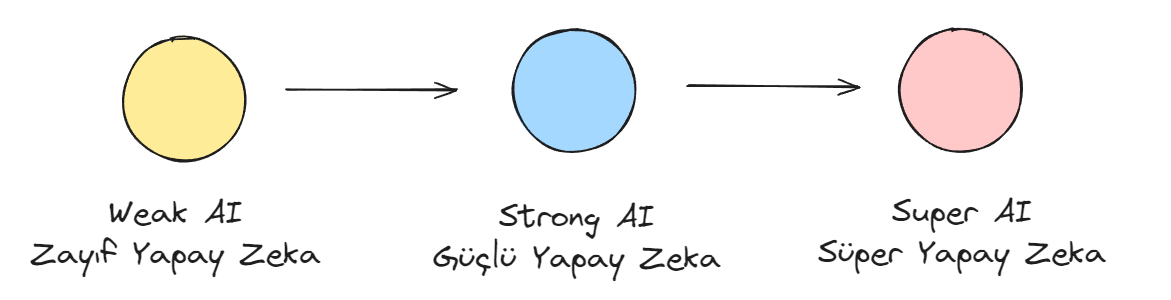
\includegraphics[width=0.8\textwidth]{images/stages_of_ai.png}
  \caption{Stages of AI.}
\end{figure}

\subsection{Zayıf Yapay Zeka (Weak AI)}
Zayıf yapay zeka, belirli bir işlevi gerçekleştirebilen, ancak başka görevler için kullanılamayan sistemlerdir. Örneğin, sesli asistanlar, oyun oynayan yapay zeka sistemleri veya öneri sistemleri zayıf yapay zeka örnekleridir. Bilinçten yoksundurlar. Sadece belirli bir görevi yapabilirler ve bu görev dışında başka görevlerde kullanılamazlar.

\subsection{Güçlü Yapay Zeka (Strong AI)}
Güçlü yapay zeka, insan zekasına benzer şekilde çeşitli görevleri gerçekleştirebilme, problem çözme yeteneğine sahip olan sistemlerdir. Bu aşamada, yapay zeka sistemleri öğrenebilir, kavrayabilir, genelleme yapabilir ve farklı alanlarda uygulanabilir. 

\subsection{Süper Yapay Zeka (Super AI)}
Süper yapay zeka, insan zekasını aşan ve daha yüksek zeka ve bilinç düzeyine sahip yapay zeka sistemleridir. Kendi kendine farkındalık geliştirebilirler. Kendi kendilerini geliştirebilirler. Güçlü yapay zeka ve süper yapay zeka hala gerçekleştirilememiştir. Üzerinde çalışmalar devam etmektedir.

\newpage